% -----------------------------*- LaTeX -*------------------------------
\documentclass[12pt]{report}


\usepackage{scribe_template}

\usepackage{hyperref}
\hypersetup{
	colorlinks=true,
	linkcolor=magenta,
	filecolor=magenta,
	citecolor = magenta,      
	urlcolor=magenta,
}
\usepackage[capitalize]{cleveref}


\begin{document}

\course{ORIE 6180}			% optional
\coursetitle{Design of Online Marketplaces} % optional
\semester{Fall 2021}			% optional
\lecturer{Sid Banerjee}		% optional
\scribe{Wolfgang Doeblin}		% required
\lecturenumber{3}			% required, must be a number
\lecturedate{August 31}		% required, omit year

\maketitle

% ----------------------------------------------------------------------


\begin{danger}
This is the danger environment.
\end{danger}

\section{Overview of the last lecture}

\section{Overview of this lecture}

\section{My first section heading}


A result from \cite{Hartline2013}, Chapter $1$. Also see \cite{Nisan2007}.

\begin{theorem}

\label{ThmNeat}
This is a neat theorem.
\end{theorem}

\begin{proof}
Lengthy and technical proof.
\begin{equation*}
\sum_{i=1}^n x_i = y.
\end{equation*}
\end{proof}



\subsection{A subsection heading}


Here is how to typeset an array of equations.

\begin{align}
	x & = y + z \nonumber \\
     E & = mc^2 \label{eq:relative}
\end{align}
You can reference equations as \cref{eq:relative}.


Here's a table.

\begin{table}[h]
\centerline{
    \begin{tabular}{|c|cc|}
	\hline
	\textbf{Method} & Cost & Iterations \\
	\hline
	Naive descent       & 12 & 200 \\
	Newton's method & 500 & 30 \\
	\hline
    \end{tabular}}
\caption{Comparison of different methods.}
\end{table}



\subsection{Yet another subsection}


\begin{corollary}
\label{CorThmNeat}
A corollary of Theorem~\ref{ThmNeat}.
\qed
\end{corollary}

\section{Some notation macros}

Use $\prn{\frac{1}{2}}$, $\crl{X|X>e^2}$ and $\brk{1-\prn{1-\frac{1}{n}}^n}$ for different braces (in order to auto-size them).

Probability notation: $\EE\brk{X\Ind_{\crl{X>y}}}$ and $\PP\brk{X>Y|Y=y}$

Typesetting linear programs:
\begin{LP}[eqn:primal-lp]{Maximize}{\sum_v r_tx_t}
  x_t \leq x_{t'} + y_{t'} + \delta_t
  & \mbox{ for all } t' \qquad\mbox{(First constraint)}\\
  x_t \leq M_t
  & \mbox{ for all } t
  \qquad\mbox{(Second constraint)}\\
  \sum_t x_t = 1 & \qquad\qquad\qquad\mbox{ (normalization)}\\
  x_t \geq 0 & \mbox{ for all } t.
\end{LP}



For figures, I would recommend coding them in a separate file in TikZ (either directly or using \href{https://www.mathcha.io/}{Mathcha} to generate TikZ code), and then importing it as in \cref{fig:bipartite}.


\begin{figure}[!tb]
	\centering
	\resizebox{0.5\textwidth}{!}{
		\tikzset{every picture/.style={line width=0.75pt}} %set default line width to 0.75pt        

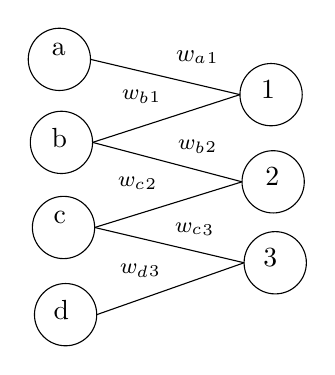
\begin{tikzpicture}[x=0.75pt,y=0.75pt,yscale=-1,xscale=1]
%uncomment if require: \path (0,300); %set diagram left start at 0, and has height of 300

%Shape: Circle [id:dp3013308924128091] 
\draw   (469,83) .. controls (469,74.72) and (475.72,68) .. (484,68) .. controls (492.28,68) and (499,74.72) .. (499,83) .. controls (499,91.28) and (492.28,98) .. (484,98) .. controls (475.72,98) and (469,91.28) .. (469,83) -- cycle ;
%Shape: Circle [id:dp48606484930054217] 
\draw   (468,43) .. controls (468,34.72) and (474.72,28) .. (483,28) .. controls (491.28,28) and (498,34.72) .. (498,43) .. controls (498,51.28) and (491.28,58) .. (483,58) .. controls (474.72,58) and (468,51.28) .. (468,43) -- cycle ;
%Shape: Circle [id:dp39812711841849757] 
\draw   (470,124) .. controls (470,115.72) and (476.72,109) .. (485,109) .. controls (493.28,109) and (500,115.72) .. (500,124) .. controls (500,132.28) and (493.28,139) .. (485,139) .. controls (476.72,139) and (470,132.28) .. (470,124) -- cycle ;
%Shape: Circle [id:dp06134916385336919] 
\draw   (471,166) .. controls (471,157.72) and (477.72,151) .. (486,151) .. controls (494.28,151) and (501,157.72) .. (501,166) .. controls (501,174.28) and (494.28,181) .. (486,181) .. controls (477.72,181) and (471,174.28) .. (471,166) -- cycle ;
%Shape: Circle [id:dp311850803690489] 
\draw   (570,60) .. controls (570,51.72) and (576.72,45) .. (585,45) .. controls (593.28,45) and (600,51.72) .. (600,60) .. controls (600,68.28) and (593.28,75) .. (585,75) .. controls (576.72,75) and (570,68.28) .. (570,60) -- cycle ;
%Shape: Circle [id:dp05972365251327605] 
\draw   (571,102) .. controls (571,93.72) and (577.72,87) .. (586,87) .. controls (594.28,87) and (601,93.72) .. (601,102) .. controls (601,110.28) and (594.28,117) .. (586,117) .. controls (577.72,117) and (571,110.28) .. (571,102) -- cycle ;
%Shape: Circle [id:dp4937409455789554] 
\draw   (572,141) .. controls (572,132.72) and (578.72,126) .. (587,126) .. controls (595.28,126) and (602,132.72) .. (602,141) .. controls (602,149.28) and (595.28,156) .. (587,156) .. controls (578.72,156) and (572,149.28) .. (572,141) -- cycle ;
%Straight Lines [id:da7683603417185125] 
\draw    (498,43) -- (570,60) ;
%Straight Lines [id:da7858813349036258] 
\draw    (499,83) -- (570,60) ;
%Straight Lines [id:da19630435102909183] 
\draw    (499,83) -- (571,102) ;
%Straight Lines [id:da7965128647751758] 
\draw    (500,124) -- (571,102) ;
%Straight Lines [id:da9969931871524618] 
\draw    (500,124) -- (572,141) ;
%Straight Lines [id:da5185515510045728] 
\draw    (501,166) -- (572,141) ;


% Text Node
\draw (478,34) node [anchor=north west][inner sep=0.75pt]   [align=left] {a};
% Text Node
\draw (478,75) node [anchor=north west][inner sep=0.75pt]   [align=left] {b};
% Text Node
\draw (479,115) node [anchor=north west][inner sep=0.75pt]   [align=left] {c};
% Text Node
\draw (479,158) node [anchor=north west][inner sep=0.75pt]   [align=left] {d};
% Text Node
\draw (579,52) node [anchor=north west][inner sep=0.75pt]   [align=left] {1};
% Text Node
\draw (581,94) node [anchor=north west][inner sep=0.75pt]   [align=left] {2};
% Text Node
\draw (580,133) node [anchor=north west][inner sep=0.75pt]   [align=left] {3};
% Text Node
\draw (538,37.4) node [anchor=north west][inner sep=0.75pt]  [font=\small]  {$w_{a}{}_{1}$};
% Text Node
\draw (512,56.4) node [anchor=north west][inner sep=0.75pt]  [font=\footnotesize]  {$w_{b}{}_{1}$};
% Text Node
\draw (539,80.4) node [anchor=north west][inner sep=0.75pt]  [font=\footnotesize]  {$w_{b}{}_{2}$};
% Text Node
\draw (510,98.4) node [anchor=north west][inner sep=0.75pt]  [font=\footnotesize]  {$w_{c}{}_{2}$};
% Text Node
\draw (537.5,120.4) node [anchor=north west][inner sep=0.75pt]  [font=\footnotesize]  {$w_{c}{}_{3}$};
% Text Node
\draw (511,140.4) node [anchor=north west][inner sep=0.75pt]  [font=\footnotesize]  {$w_{d}{}_{3}$};
\end{tikzpicture}
\tikzset{every picture/.style={line width=0.75pt}} %set default line width to 0.75pt        

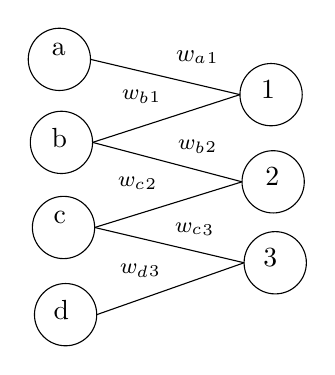
\begin{tikzpicture}[x=0.75pt,y=0.75pt,yscale=-1,xscale=1]
%uncomment if require: \path (0,300); %set diagram left start at 0, and has height of 300

%Shape: Circle [id:dp3013308924128091] 
\draw   (469,83) .. controls (469,74.72) and (475.72,68) .. (484,68) .. controls (492.28,68) and (499,74.72) .. (499,83) .. controls (499,91.28) and (492.28,98) .. (484,98) .. controls (475.72,98) and (469,91.28) .. (469,83) -- cycle ;
%Shape: Circle [id:dp48606484930054217] 
\draw   (468,43) .. controls (468,34.72) and (474.72,28) .. (483,28) .. controls (491.28,28) and (498,34.72) .. (498,43) .. controls (498,51.28) and (491.28,58) .. (483,58) .. controls (474.72,58) and (468,51.28) .. (468,43) -- cycle ;
%Shape: Circle [id:dp39812711841849757] 
\draw   (470,124) .. controls (470,115.72) and (476.72,109) .. (485,109) .. controls (493.28,109) and (500,115.72) .. (500,124) .. controls (500,132.28) and (493.28,139) .. (485,139) .. controls (476.72,139) and (470,132.28) .. (470,124) -- cycle ;
%Shape: Circle [id:dp06134916385336919] 
\draw   (471,166) .. controls (471,157.72) and (477.72,151) .. (486,151) .. controls (494.28,151) and (501,157.72) .. (501,166) .. controls (501,174.28) and (494.28,181) .. (486,181) .. controls (477.72,181) and (471,174.28) .. (471,166) -- cycle ;
%Shape: Circle [id:dp311850803690489] 
\draw   (570,60) .. controls (570,51.72) and (576.72,45) .. (585,45) .. controls (593.28,45) and (600,51.72) .. (600,60) .. controls (600,68.28) and (593.28,75) .. (585,75) .. controls (576.72,75) and (570,68.28) .. (570,60) -- cycle ;
%Shape: Circle [id:dp05972365251327605] 
\draw   (571,102) .. controls (571,93.72) and (577.72,87) .. (586,87) .. controls (594.28,87) and (601,93.72) .. (601,102) .. controls (601,110.28) and (594.28,117) .. (586,117) .. controls (577.72,117) and (571,110.28) .. (571,102) -- cycle ;
%Shape: Circle [id:dp4937409455789554] 
\draw   (572,141) .. controls (572,132.72) and (578.72,126) .. (587,126) .. controls (595.28,126) and (602,132.72) .. (602,141) .. controls (602,149.28) and (595.28,156) .. (587,156) .. controls (578.72,156) and (572,149.28) .. (572,141) -- cycle ;
%Straight Lines [id:da7683603417185125] 
\draw    (498,43) -- (570,60) ;
%Straight Lines [id:da7858813349036258] 
\draw    (499,83) -- (570,60) ;
%Straight Lines [id:da19630435102909183] 
\draw    (499,83) -- (571,102) ;
%Straight Lines [id:da7965128647751758] 
\draw    (500,124) -- (571,102) ;
%Straight Lines [id:da9969931871524618] 
\draw    (500,124) -- (572,141) ;
%Straight Lines [id:da5185515510045728] 
\draw    (501,166) -- (572,141) ;


% Text Node
\draw (478,34) node [anchor=north west][inner sep=0.75pt]   [align=left] {a};
% Text Node
\draw (478,75) node [anchor=north west][inner sep=0.75pt]   [align=left] {b};
% Text Node
\draw (479,115) node [anchor=north west][inner sep=0.75pt]   [align=left] {c};
% Text Node
\draw (479,158) node [anchor=north west][inner sep=0.75pt]   [align=left] {d};
% Text Node
\draw (579,52) node [anchor=north west][inner sep=0.75pt]   [align=left] {1};
% Text Node
\draw (581,94) node [anchor=north west][inner sep=0.75pt]   [align=left] {2};
% Text Node
\draw (580,133) node [anchor=north west][inner sep=0.75pt]   [align=left] {3};
% Text Node
\draw (538,37.4) node [anchor=north west][inner sep=0.75pt]  [font=\small]  {$w_{a}{}_{1}$};
% Text Node
\draw (512,56.4) node [anchor=north west][inner sep=0.75pt]  [font=\footnotesize]  {$w_{b}{}_{1}$};
% Text Node
\draw (539,80.4) node [anchor=north west][inner sep=0.75pt]  [font=\footnotesize]  {$w_{b}{}_{2}$};
% Text Node
\draw (510,98.4) node [anchor=north west][inner sep=0.75pt]  [font=\footnotesize]  {$w_{c}{}_{2}$};
% Text Node
\draw (537.5,120.4) node [anchor=north west][inner sep=0.75pt]  [font=\footnotesize]  {$w_{c}{}_{3}$};
% Text Node
\draw (511,140.4) node [anchor=north west][inner sep=0.75pt]  [font=\footnotesize]  {$w_{d}{}_{3}$};
\end{tikzpicture}

	}
	\caption{\em A friendly weighted bipartite graph}
	\label{fig:bipartite}
\end{figure}





\begin{thebibliography}{1}

\bibitem{Hartline2013}
{\sc Hartline, J.~D.}
\newblock Mechanism design and approximation.

\bibitem{Nisan2007}
{\sc Nisan, N., Roughgarden, T., Tardos, E., and Vazirani, V.~V.}
\newblock {\em Algorithmic game theory}, vol.~1.
\newblock Cambridge University Press Cambridge, 2007.

\end{thebibliography}

\end{document}


